\documentclass{article}

\usepackage{hyperref}
\usepackage{xcolor}
\usepackage{pdfpages}
\usepackage[spanish]{babel}
\usepackage{graphicx}

\title{Entrega 2}
\author{Grupo 131 \\ Leopoldo Farr \\ Benjamin Huenchuñir}
\date{\today}

\begin{document}

\maketitle

\section{Diagrama E/R}

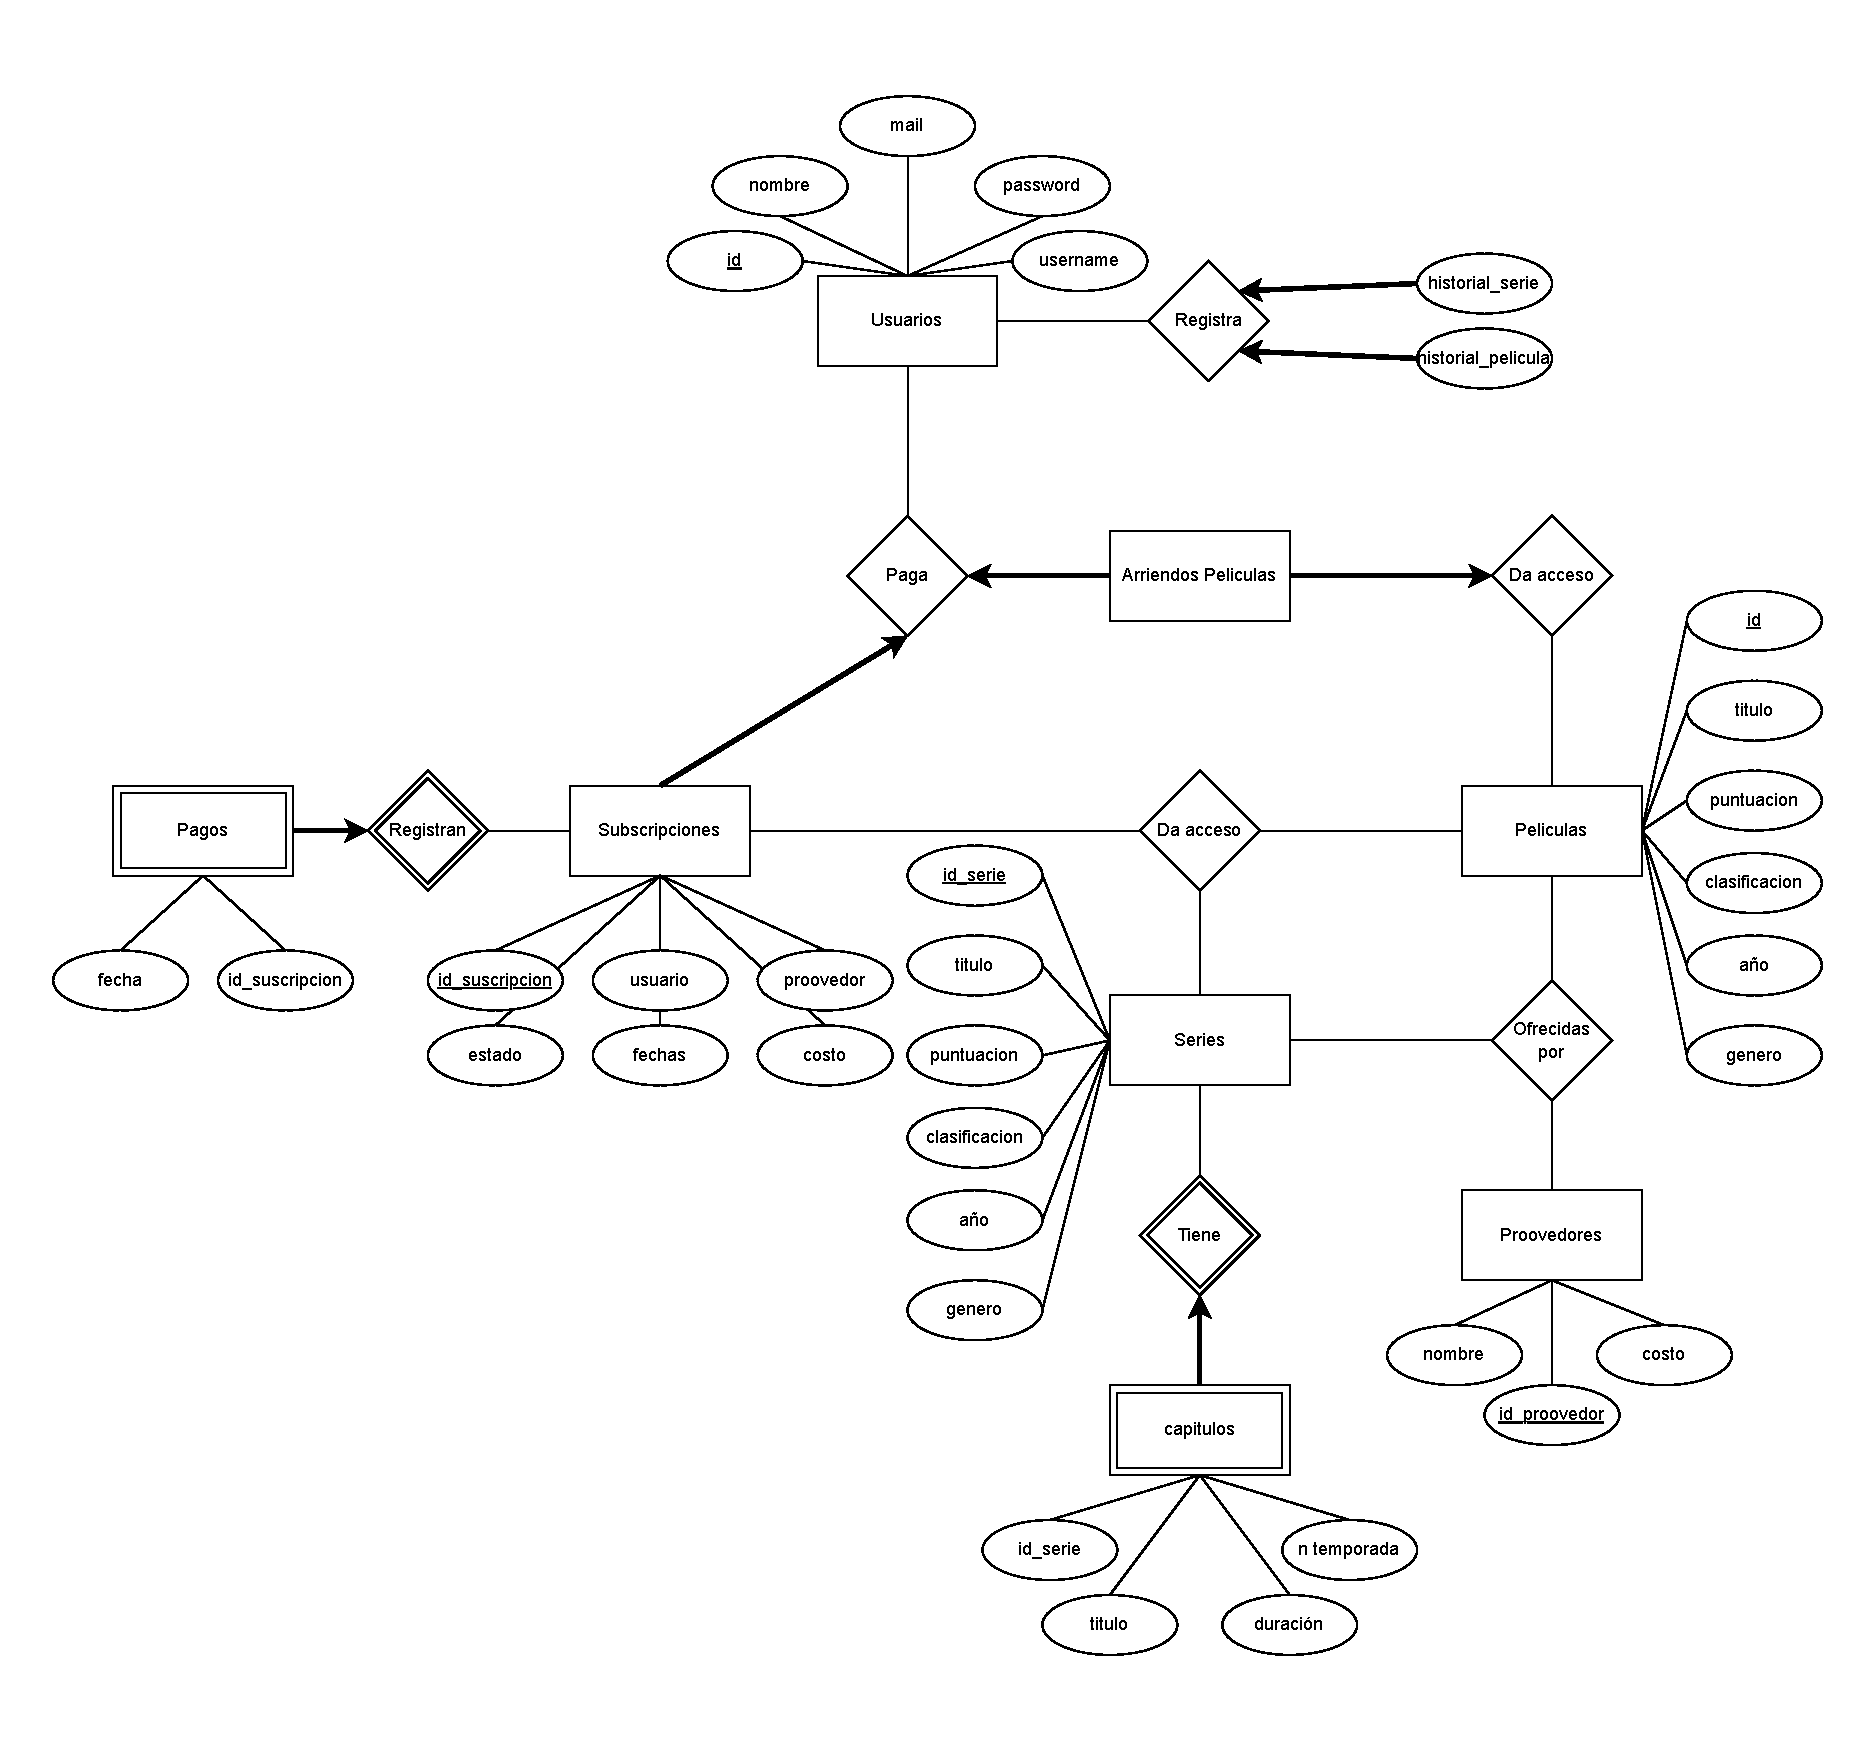
\includegraphics[width=16cm]{Esquemas/diagrama_ER.pdf}

\section{Esquema relacional}

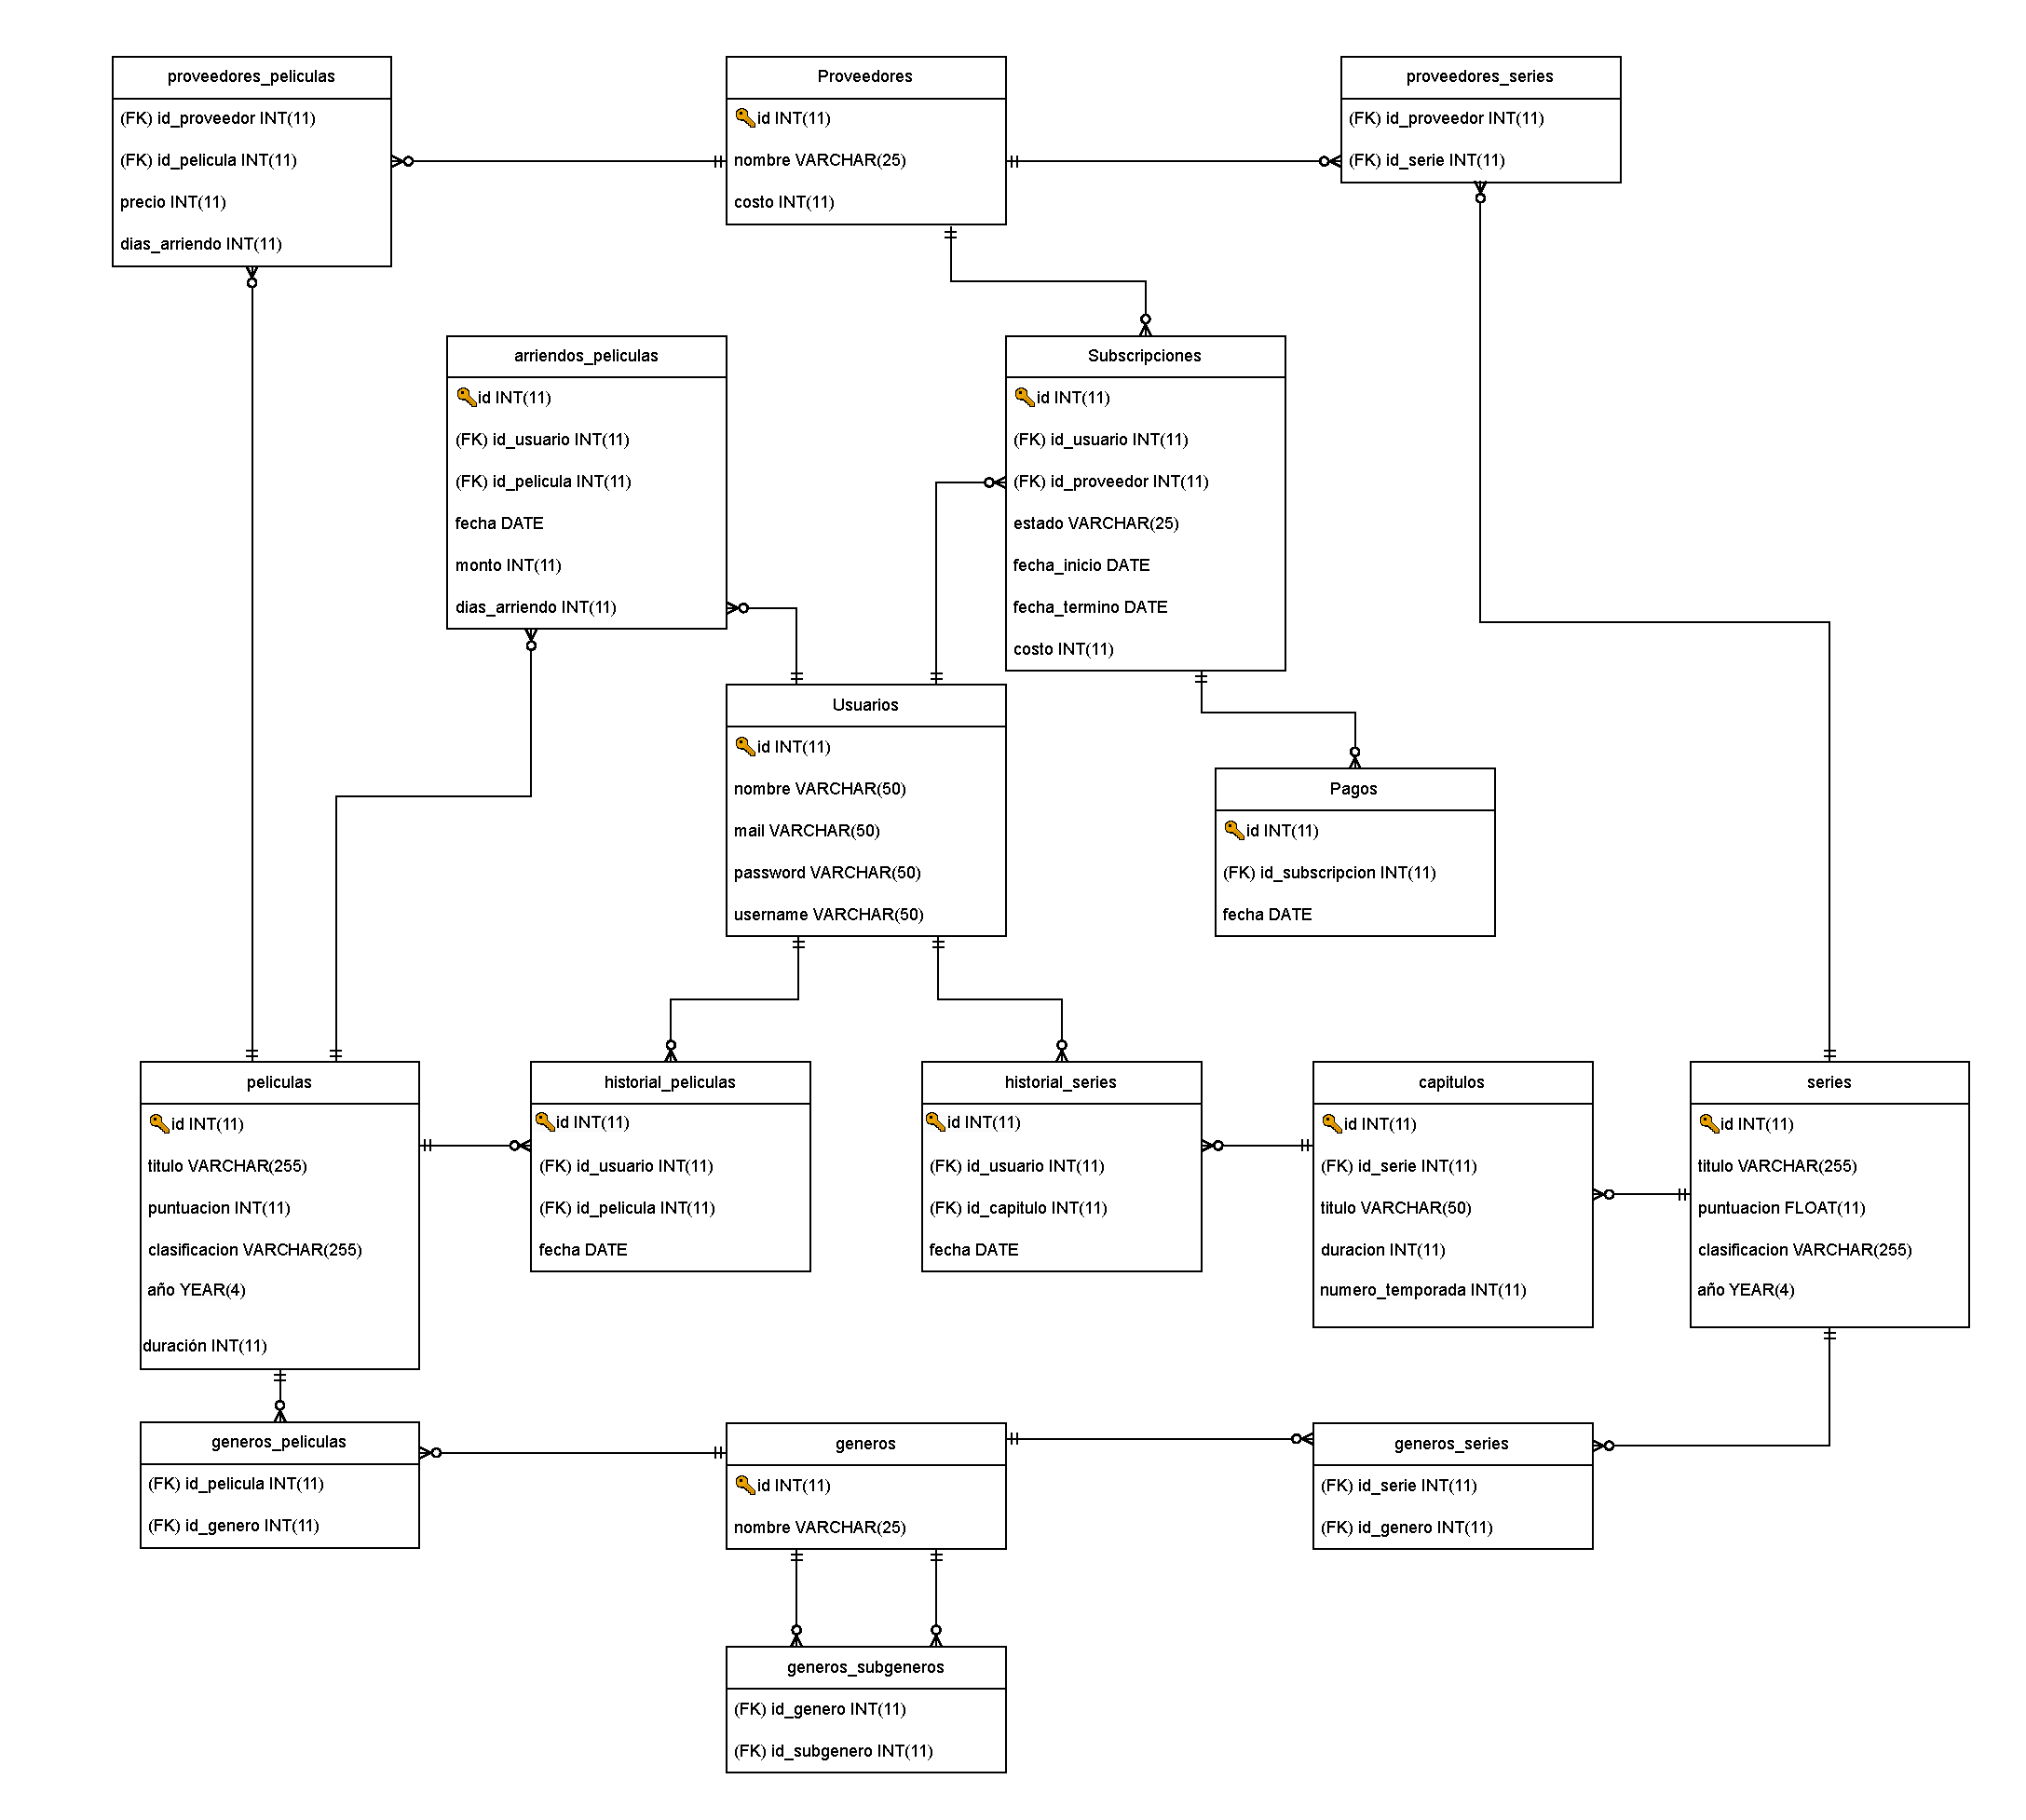
\includegraphics[width=16cm]{Esquemas/EsquemaRelacionalFinal.pdf}

\section{Dependencias funcionales y justificación}
\begin{enumerate}
    \item proveedores\_peliculas \\
    Las dependencias de esta tabla están en BCNF dado que no existen repeticiones de datos y cada columna depende unicamente de la llave mínimal de la siguiente forma: \\
    id\_proveedor, id\_pelicula $\rightarrow$ precio, dias\_arriendo
    \item Proveedores \\
    Las dependencias de esta tabla están en BCNF dado que no existen repeticiones de datos y cada columna depende unicamente de la llave mínimal de la siguiente forma: \\
    id $\rightarrow$ nombre, costo
    \item proveedores\_series \\
    Las dependencias de esta tabla están en BCNF dado que no existen repeticiones de datos y cada columna es independiente, por lo que no existen dependencias que transgredan BCNF. \\
    \item arriendos\_peliculas \\
    Las dependencias de esta tabla están en BCNF dado que no existen repeticiones de datos y cada columna depende unicamente de la llave mínimal de la siguiente forma: \\
    id $\rightarrow$ id\_usuario, id\_pelicula, fecha, monto, dias\_arriendo \\
    \item Subscripciones \\
    Las dependencias de esta tabla están en BCNF dado que no existen repeticiones de datos y cada columna depende unicamente de la llave mínimal de la siguiente forma: \\
    id $\rightarrow$ id\_usuario, id\_proveedor, estado, fecha\_inicio, fecha\_termino, costo \\
    \item Usuarios \\
    Las dependencias de esta tabla están en BCNF dado que no existen repeticiones de datos y cada columna depende unicamente de la llave mínimal de la siguiente forma: \\
    id $\rightarrow$ nombre, mail, password, username \\
    \item Pagos \\
    Las dependencias de esta tabla están en BCNF dado que no existen repeticiones de datos y cada columna depende unicamente de la llave mínimal de la siguiente forma: \\
    id $\rightarrow$ id\_subscripcion, fecha \\
    \item peliculas \\
    Las dependencias de esta tabla están en BCNF dado que no existen repeticiones de datos y cada columna depende unicamente de la llave mínimal de la siguiente forma: \\
    id $\rightarrow$ titulo, puntuacion, clasificacion, año, duracion \\
    \item historial\_peliculas \\
    Las dependencias de esta tabla están en BCNF dado que no existen repeticiones de datos y cada columna depende unicamente de la llave mínimal de la siguiente forma: \\
    id $\rightarrow$ id\_usuario, id\_pelicula, fecha \\
    \item historial\_series \\
    Las dependencias de esta tabla están en BCNF dado que no existen repeticiones de datos y cada columna depende unicamente de la llave mínimal de la siguiente forma: \\
    id $\rightarrow$ id\_usuario, id\_capitulo, fecha \\
    \item capitulos \\
    Las dependencias de esta tabla están en BCNF dado que no existen repeticiones de datos y cada columna depende unicamente de la llave mínimal de la siguiente forma: \\
    id $\rightarrow$ id\_serie, titulo, duracion, numero\_temporada \\
    \item series \\
    Las dependencias de esta tabla están en BCNF dado que no existen repeticiones de datos y cada columna depende unicamente de la llave mínimal de la siguiente forma: \\
    id $\rightarrow$ titulo, puntuacion, clasificacion, año \\
    \item generos\_peliculas \\
    Las dependencias de esta tabla están en BCNF dado que no existen repeticiones de datos y cada columna es independiente, por lo que no existen dependencias que transgredan BCNF. \\
     \item generos \\
    Las dependencias de esta tabla están en BCNF dado que no existen repeticiones de datos y cada columna depende unicamente de la llave mínimal de la siguiente forma: \\
    id $\rightarrow$ nombre \\
    \item generos\_series \\
    Las dependencias de esta tabla están en BCNF dado que no existen repeticiones de datos y cada columna es independiente, por lo que no existen dependencias que transgredan BCNF. \\
    \item generos\_subgeneros\\
    Las dependencias de esta tabla están en BCNF dado que no existen repeticiones de datos y cada columna es independiente, por lo que no existen dependencias que transgredan BCNF. \\
\end{enumerate}

\section{Consultas}
\begin{enumerate}
    \item \textbf{Muestre todas las películas junto con sus proveedores, siempre y cuando el proveedor las ofrezca de manera gratuita} \\
    SELECT peliculas.titulo AS pelicula, proveedores.nombre AS proveedor FROM peliculas
    INNER JOIN proveedores\_peliculas ON peliculas.id = proveedores\_peliculas.id\_pelicula
    INNER JOIN proveedores ON proveedores\_peliculas.id\_proveedor = proveedores.id
    WHERE proveedores\_peliculas.precio IS NULL;
    \item \textbf{Dado un numero n ingresado por el usuario, muestre todas las series que tengan al menos n temporadas} \\
    SELECT series.titulo AS serie, COUNT(DISTINCT capitulos.numero\_temporada) AS cantidad\_temporadas FROM series
    INNER JOIN capitulos ON series.id = capitulos.id\_serie
    GROUP BY series.id, series.titulo
    HAVING COUNT(DISTINCT capitulos.numero\_temporada) $>$= \textcolor{cyan}{numero\_temporadas};
    \item \textbf{Dado un titulo ingresado por el usuario, muestre todas las películas/series con ese título y los proveedores que las ofrecen} \\
    SELECT * FROM (
        SELECT peliculas.titulo AS titulo, proveedores.nombre AS proveedor FROM peliculas
        INNER JOIN proveedores\_peliculas ON peliculas.id = proveedores\_peliculas.id\_pelicula
        INNER JOIN proveedores ON proveedores\_peliculas.id\_proveedor = proveedores.id
        UNION
        SELECT series.titulo AS titulo, proveedores.nombre AS proveedor FROM series
        INNER JOIN proveedores\_series ON series.id = proveedores\_series.id\_serie
        INNER JOIN proveedores ON proveedores\_series.id\_proveedor = proveedores.id
    ) AS U WHERE UPPER(titulo) = UPPER(\textcolor{cyan}{titulo\_pelicula});
    \item \textbf{Dado un genero seleccionado por el usuario, muestre todas las películas que pertenezcan a ese género, o que pertenezcan a alguno de sus subgéneros inmediatos} \\
    SELECT DISTINCT peliculas.titulo AS titulo, generos.nombre AS genero FROM peliculas
    INNER JOIN generos\_peliculas ON peliculas.id = generos\_peliculas.id\_pelicula
    INNER JOIN generos ON generos\_peliculas.id\_genero = generos.id
    WHERE generos\_peliculas.id\_genero = \textcolor{cyan}{id\_genero}
    OR generos\_peliculas.id\_genero IN (
        SELECT id\_subgenero FROM genero\_subgeneros WHERE id\_genero = \textcolor{cyan}{id\_genero}
    );
\newpage
    \item \textbf{Dado un username ingresado por el usuario, muestre todas las películas a las que tiene acceso dicho usuario} \\
    SELECT DISTINCT peliculas.titulo AS pelicula FROM peliculas
    INNER JOIN proveedores\_peliculas ON peliculas.id = proveedores\_peliculas.id\_pelicula
    INNER JOIN subscripciones ON proveedores\_peliculas.id\_proveedor = subscripciones.id\_proveedor
    INNER JOIN usuarios ON subscripciones.id\_usuario = usuarios.id
    LEFT JOIN arriendos\_peliculas ON peliculas.id = arriendos\_peliculas.id\_pelicula AND arriendos\_peliculas.id\_usuario = usuarios.id
    WHERE UPPER(usuarios.username) = UPPER(\textcolor{cyan}{username})
    AND (
        (precio IS NULL AND subscripciones.fecha\_termino IS NULL)
        OR
        (precio IS NOT NULL AND arriendos\_peliculas.id IS NOT NULL AND (CURRENT\_DATE $<$= arriendos\_peliculas.fecha + arriendos\_peliculas.dias\_arriendo))
    );
    \item \textbf{Dado un username ingresado por el usuario, muestre todas las series para las cuales el usuario ingresado ha visto mas de un capítulo en el último año} \\
    SELECT series.titulo AS titulo, COUNT(*) AS cantidad\_capitulos FROM historial\_series
    INNER JOIN capitulos ON historial\_series.id\_capitulo = capitulos.id
    INNER JOIN series ON series.id = capitulos.id\_serie
    INNER JOIN usuarios ON historial\_series.id\_usuario = usuarios.id
    WHERE UPPER(usuarios.username) = UPPER(\textcolor{cyan}{username})
    AND historial\_series.fecha $>$= CURRENT\_DATE - INTERVAL '4 year'
    GROUP BY series.id, series.titulo
    HAVING COUNT(*) $>$ 1;
    \item \textbf{Muestre la suma de dinero gastada por cada usuario en películas no incluidas en planes de suscripción} \\
    SELECT usuarios.nombre AS usuario, SUM(arriendos\_peliculas.monto) AS total FROM arriendos\_peliculas
    INNER JOIN usuarios ON arriendos\_peliculas.id\_usuario = usuarios.id
    GROUP BY usuarios.id, usuarios.nombre;
\end{enumerate}

\section{Supuestos}
\begin{enumerate}
    \item Para la consulta 6, "Dado un username ingresado por el usuario, muestre todas las series para las cuales el usuario ha visto más de un capítulo durante el último año", el ver dos veces el mismo capítulo también cuenta (issue \href{https://github.com/IIC2413/Syllabus-2023-2/issues/172}{\#72}).
    \item Para las consultas que piden "en el ultimo año" se consideró un intervalo de tiempo mayor (4 años), ya que no hay datos del último año (issue \href{https://github.com/IIC2413/Syllabus-2023-2/issues/175}{\#175})
    \item Clasificación, puntuación y año son de la serie y no varían según capítulo (issue \href{https://github.com/IIC2413/Syllabus-2023-2/issues/171}{\#171})
    \item La serie "Rick  y Morty" no tiene género en los datos entregados, se le asignó "Comedia" (issue \href{https://github.com/IIC2413/Syllabus-2023-2/issues/189}{\#189})
    \item Se eliminó el atributo "estado" de la tabla de subscripciones, ya que solo representa si la subscripción esta activa o no, y eso se puede inferir de la fecha de termino (si existe o es nula). Así se evita una dependencia transitiva.
    \item Al igual que el costo de subscripción y el costo de arriendo de una película, los días de arriendo de la película (el atributo "disponibilidad") también pueden variar en el tiempo, requiriendo ser guardados para cada arriendo.
    \item Una serie que tiene capítulos pertenecientes a n temporadas distintas tiene n temporadas, sin importar el número de temporada de estas (issue \href{https://github.com/IIC2413/Syllabus-2023-2/issues/200}{\#200})
\end{enumerate}


\end{document}
